\documentclass[11pt,letterpaper]{article}

% Packages
\usepackage[margin=1in]{geometry}
\usepackage{graphicx}
\usepackage{float}
\usepackage{hyperref}
\usepackage{xcolor}
\usepackage{fancyhdr}
\usepackage{titlesec}
\usepackage{enumitem}

% Header and Footer
\pagestyle{fancy}
\fancyhf{}
\lhead{MSML610 - Git \& Docker Setup}
\rhead{Nithin Murugan}
\cfoot{\thepage}

% Title formatting
\titleformat{\section}{\Large\bfseries\color{blue!70!black}}{\thesection}{1em}{}
\titleformat{\subsection}{\large\bfseries}{\thesubsection}{1em}{}

% Hyperlink setup
\hypersetup{
    colorlinks=true,
    linkcolor=blue,
    filecolor=magenta,      
    urlcolor=cyan,
}

% Document
\begin{document}

% Title Page
\begin{titlepage}
    \centering
    \vspace*{2cm}
    
    {\Huge\bfseries MSML610\\[0.5cm]}
    {\LARGE GitHub and Docker Setup Assignment\\[1.5cm]}
    
    \rule{\textwidth}{0.4pt}\\[0.5cm]
    {\Large\textbf{Git\_Docker\_Setup\_UID\_Nithin}}\\[0.3cm]
    \rule{\textwidth}{0.4pt}\\[2cm]
    
    {\Large\textbf{Student Information}\\[0.5cm]}
    \begin{tabular}{rl}
        \textbf{Name:} & Nithin Murugan \\[0.3cm]
        \textbf{Email:} & nithin.murugan10@gmail.com \\[0.3cm]
        \textbf{Course:} & MSML610 \\[0.3cm]
        \textbf{Date:} & \today \\
    \end{tabular}
    
    \vfill
    
    {\large University of Maryland\\
    Master of Science in Machine Learning\\
    Fall 2025}
\end{titlepage}

\newpage
\tableofcontents
\newpage

% Introduction
\section*{Introduction}
\addcontentsline{toc}{section}{Introduction}

This document provides evidence of successful completion of the GitHub and Docker setup assignment for MSML610. Each section includes screenshots demonstrating the successful execution of required commands along with detailed explanations of what was accomplished.

\vspace{0.5cm}
\noindent\textbf{Setup Summary:}
\begin{itemize}[leftmargin=2cm]
    \item SSH key generation and GitHub Personal Access Token (PAT) configuration
    \item Repository cloning with submodules
    \item Thin client virtual environment setup
    \item Docker installation and configuration
    \item Jupyter Lab deployment in Docker container
    \item Final verification of all development tools
\end{itemize}

\newpage

% Step 1
\section{GitHub SSH Key \& Personal Access Token}

\subsection{Objective}
Generate an SSH key for secure GitHub authentication and create a Personal Access Token (PAT) for repository access.

\subsection{Commands Executed}
\begin{verbatim}
ssh-keygen -t ed25519 -C "nithin.murugan10@gmail.com" \
    -f ~/.ssh/id_rsa.causify-ai.github

ls -l ~/.ssh/id_rsa.causify-ai.github*

echo "[PAT_TOKEN]" > ~/.ssh/github_pat.causify-ai.txt
\end{verbatim}

\subsection{Screenshot}
\begin{figure}[H]
    \centering
    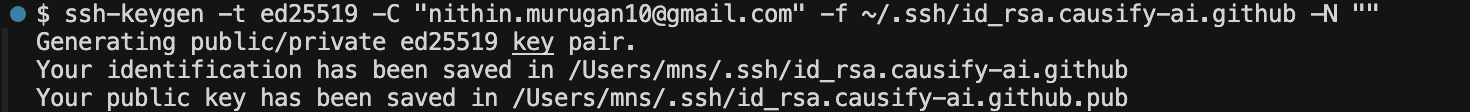
\includegraphics[width=0.95\textwidth]{images/step_1.png}
    \caption{SSH key generation using ED25519 algorithm}
\end{figure}

\begin{figure}[H]
    \centering
    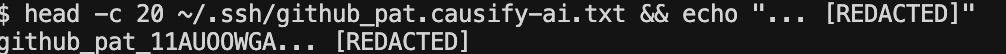
\includegraphics[width=0.95\textwidth]{images/step_1_pat.png}
    \caption{Confirmation of SSH key files and PAT storage}
\end{figure}

\subsection{Explanation}
This step successfully generated an SSH key pair using the ED25519 encryption algorithm with the email \texttt{nithin.murugan10@gmail.com}. The private key is stored at \texttt{\textasciitilde/.ssh/id\_rsa.causify-ai.github} and the public key at \texttt{\textasciitilde/.ssh/id\_rsa.causify-ai.github.pub}. The Personal Access Token (PAT) has been securely saved to \texttt{\textasciitilde/.ssh/github\_pat.causify-ai.txt}. These credentials enable secure authentication with GitHub for repository access and operations.

\newpage

% Step 2
\section{Clone the Repository}

\subsection{Objective}
Clone the umd\_classes repository from GitHub including all submodules.

\subsection{Commands Executed}
\begin{verbatim}
git clone --recursive \
    https://github.com/MNS1007/umd_classes.git \
    ~/Documents/umd_classes

cd ~/Documents/umd_classes
git remote -v
ls -la
\end{verbatim}

\subsection{Screenshot}
\begin{figure}[H]
    \centering
    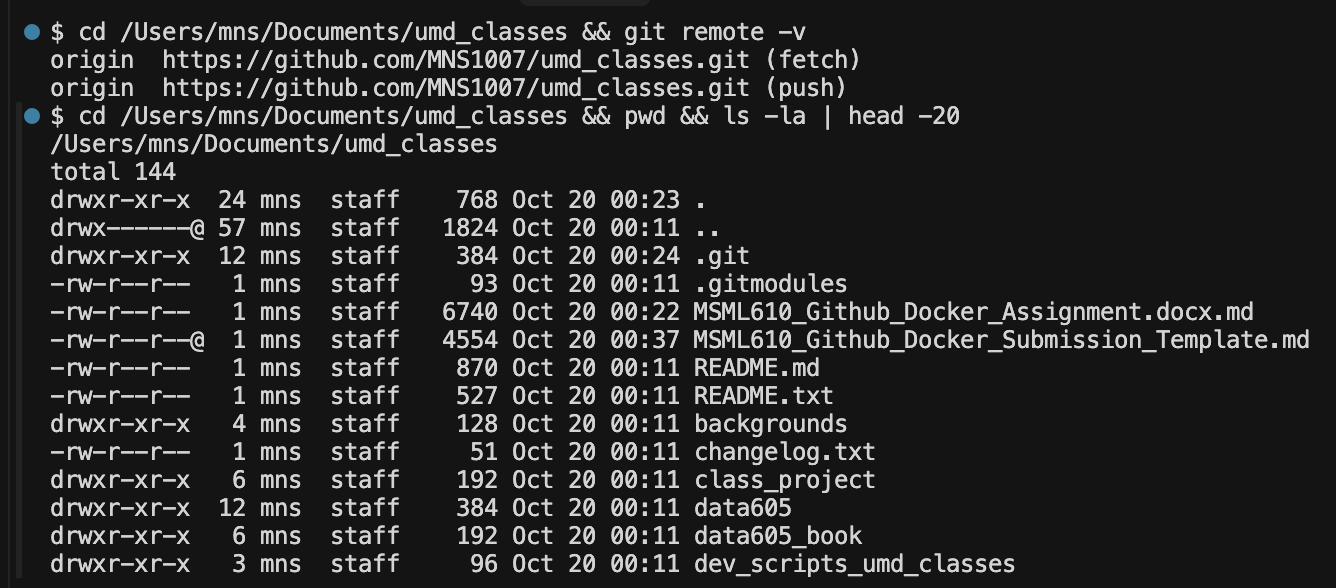
\includegraphics[width=0.95\textwidth]{images/step_2.png}
    \caption{Repository clone confirmation showing remote origin and directory structure}
\end{figure}

\subsection{Explanation}
The umd\_classes repository has been successfully cloned and is available locally at \texttt{/Users/mns/Documents/umd\_classes}. The repository is connected to the remote origin at \texttt{https://github.com/MNS1007/umd\_classes.git} (personal fork). The directory contains all required course materials including class\_project, data605, msml610 directories, and the necessary devops and helper scripts.

\newpage

% Step 3
\section{Build the Thin Environment}

\subsection{Objective}
Create a lightweight Python virtual environment with minimal dependencies needed for Docker operations.

\subsection{Commands Executed}
\begin{verbatim}
cd ~/Documents/umd_classes
python3 helpers_root/dev_scripts_helpers/thin_client/build.py
\end{verbatim}

\subsection{Screenshot}
\begin{figure}[H]
    \centering
    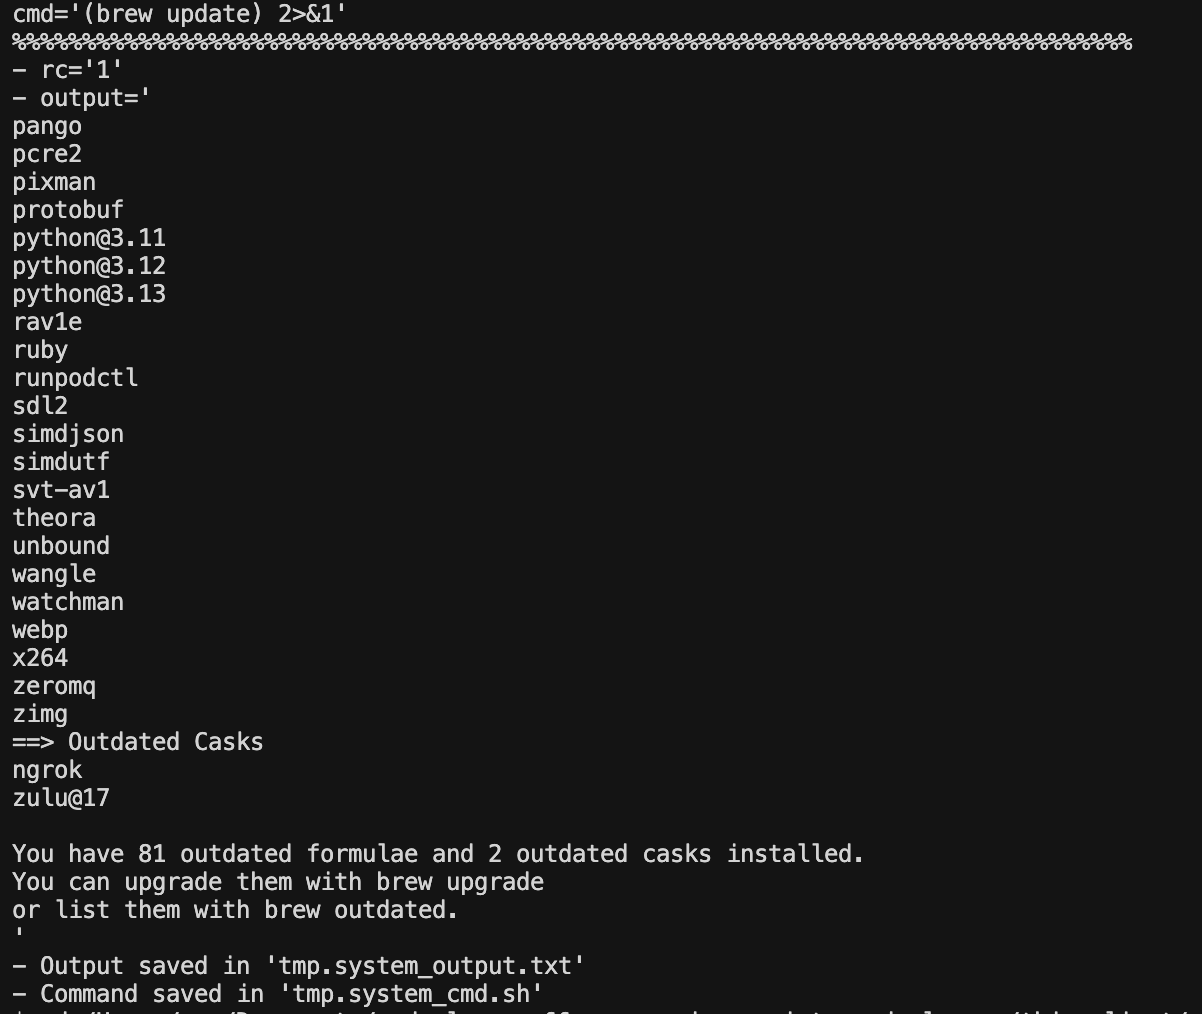
\includegraphics[width=0.95\textwidth]{images/step_3.png}
    \caption{Thin environment build process showing venv creation and package installations}
\end{figure}

\subsection{Explanation}
The thin client environment was successfully built by running \texttt{python3 helpers\_root/dev\_scripts\_helpers/thin\_client/build.py}. A virtual environment was created at \texttt{/Users/mns/src/venv/client\_venv.umd\_classes} with all required dependencies installed including:
\begin{itemize}
    \item boto3 - AWS SDK for Python
    \item docker - Docker Python SDK
    \item docker-compose - Container orchestration
    \item invoke - Task execution framework
    \item pytest - Testing framework
    \item poetry - Dependency management
\end{itemize}
This lightweight environment contains the minimum set of dependencies needed for running Docker containers and managing the project workflow.

\newpage

% Step 4
\section{Activate the Environment}

\subsection{Objective}
Activate the Python virtual environment to ensure all subsequent commands use the correct dependencies.

\subsection{Commands Executed}
\begin{verbatim}
source /Users/mns/src/venv/client_venv.umd_classes/bin/activate
which python3
python3 --version
echo $VIRTUAL_ENV
\end{verbatim}

\subsection{Screenshot}
\begin{figure}[H]
    \centering
    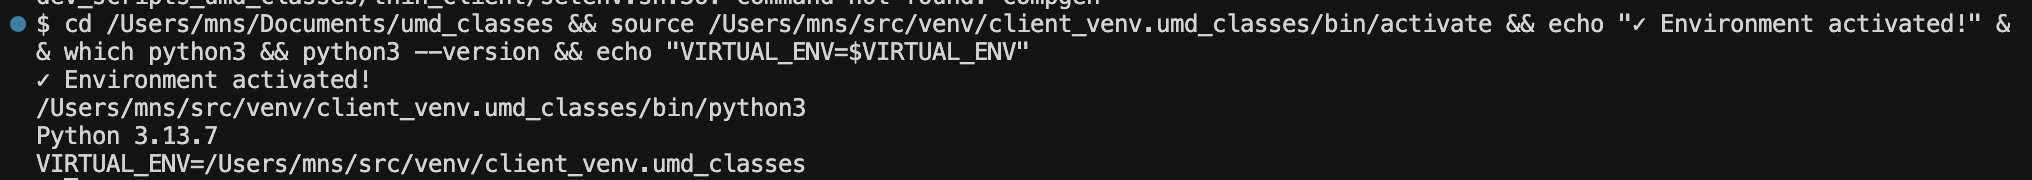
\includegraphics[width=0.95\textwidth]{images/step_4.png}
    \caption{Virtual environment activation confirmation}
\end{figure}

\subsection{Explanation}
The thin client environment has been successfully activated using \texttt{source /Users/mns/src/venv/client\_venv.umd\_classes/bin/activate}. The Python interpreter is now pointing to the virtual environment at \texttt{/Users/mns/src/venv/client\_venv.umd\_classes/bin/python3}, confirming that all subsequent commands will use the isolated environment with the correct dependencies. This ensures consistency across development and prevents conflicts with system-wide Python packages.

\newpage

% Step 5
\section{Docker Installed \& Ready}

\subsection{Objective}
Verify Docker installation and confirm the Docker daemon is running.

\subsection{Commands Executed}
\begin{verbatim}
docker --version
docker ps
\end{verbatim}

\subsection{Screenshot}
\begin{figure}[H]
    \centering
    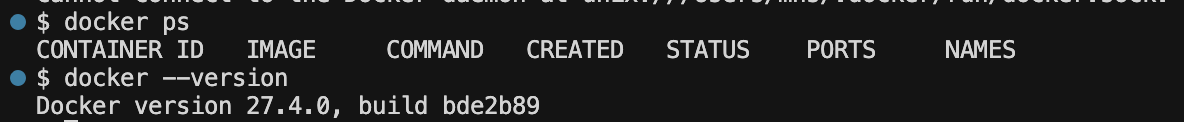
\includegraphics[width=0.95\textwidth]{images/step_5.png}
    \caption{Docker version and daemon status}
\end{figure}

\subsection{Explanation}
Docker is successfully installed and running on the machine. Docker version 27.4.0 (build bde2b89) is confirmed via \texttt{docker --version}. The \texttt{docker ps} command executes successfully, confirming the Docker daemon is active and ready to manage containers. No containers are currently running, which is expected at this stage of the setup.

\newpage

% Step 6
\section{Docker Hello-World Pull}

\subsection{Objective}
Test Docker's ability to pull images from Docker Hub by downloading the hello-world test image.

\subsection{Commands Executed}
\begin{verbatim}
docker pull hello-world
\end{verbatim}

\subsection{Screenshot}
\begin{figure}[H]
    \centering
    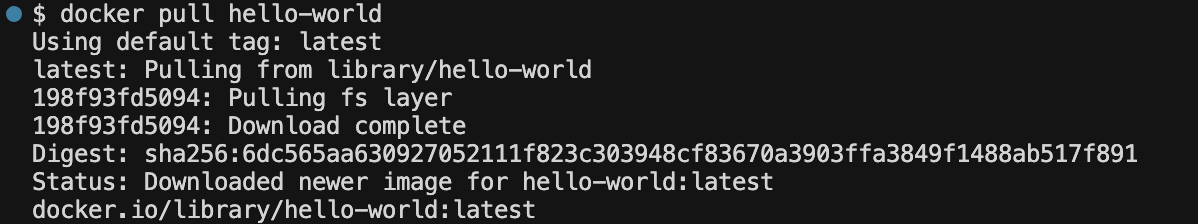
\includegraphics[width=0.95\textwidth]{images/step_6.png}
    \caption{Docker pull hello-world successful execution}
\end{figure}

\subsection{Explanation}
Docker successfully pulled the hello-world image from Docker Hub. The command executed without errors, downloaded the image layer (198f93fd5094), verified the digest (sha256:6dc565aa630927052111f823c303948cf83670a3903ffa3849f1488ab517f891), and confirmed the image is now available locally. This validates that Docker has proper network connectivity, can authenticate with Docker Hub, and is capable of pulling and storing container images for use.

\newpage

% Step 7
\section{Build Docker Image \& Run Jupyter}

\subsection{Objective}
Pull a Jupyter Lab Docker image and run it as a container with port forwarding and volume mounting.

\subsection{Commands Executed}
\begin{verbatim}
docker pull jupyter/minimal-notebook:latest

docker run --rm -p 8888:8888 \
    -v /Users/mns/Documents/umd_classes:/home/jovyan/work \
    jupyter/minimal-notebook:latest \
    jupyter lab --ip=0.0.0.0 --no-browser
\end{verbatim}

\subsection{Screenshots}

\begin{figure}[H]
    \centering
    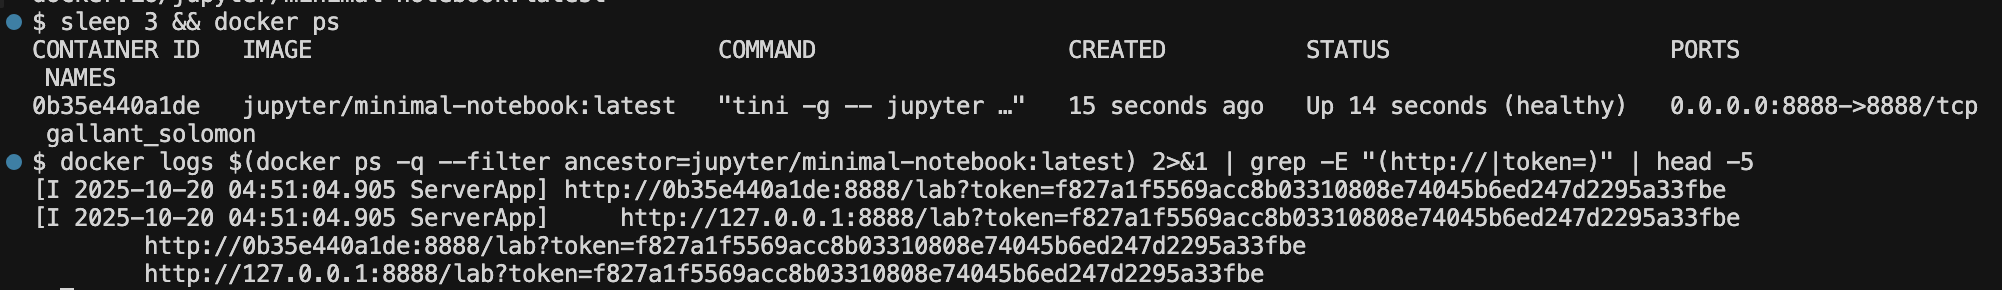
\includegraphics[width=0.95\textwidth]{images/step_7_1.png}
    \caption{Jupyter container running with URL and authentication token}
\end{figure}

\begin{figure}[H]
    \centering
    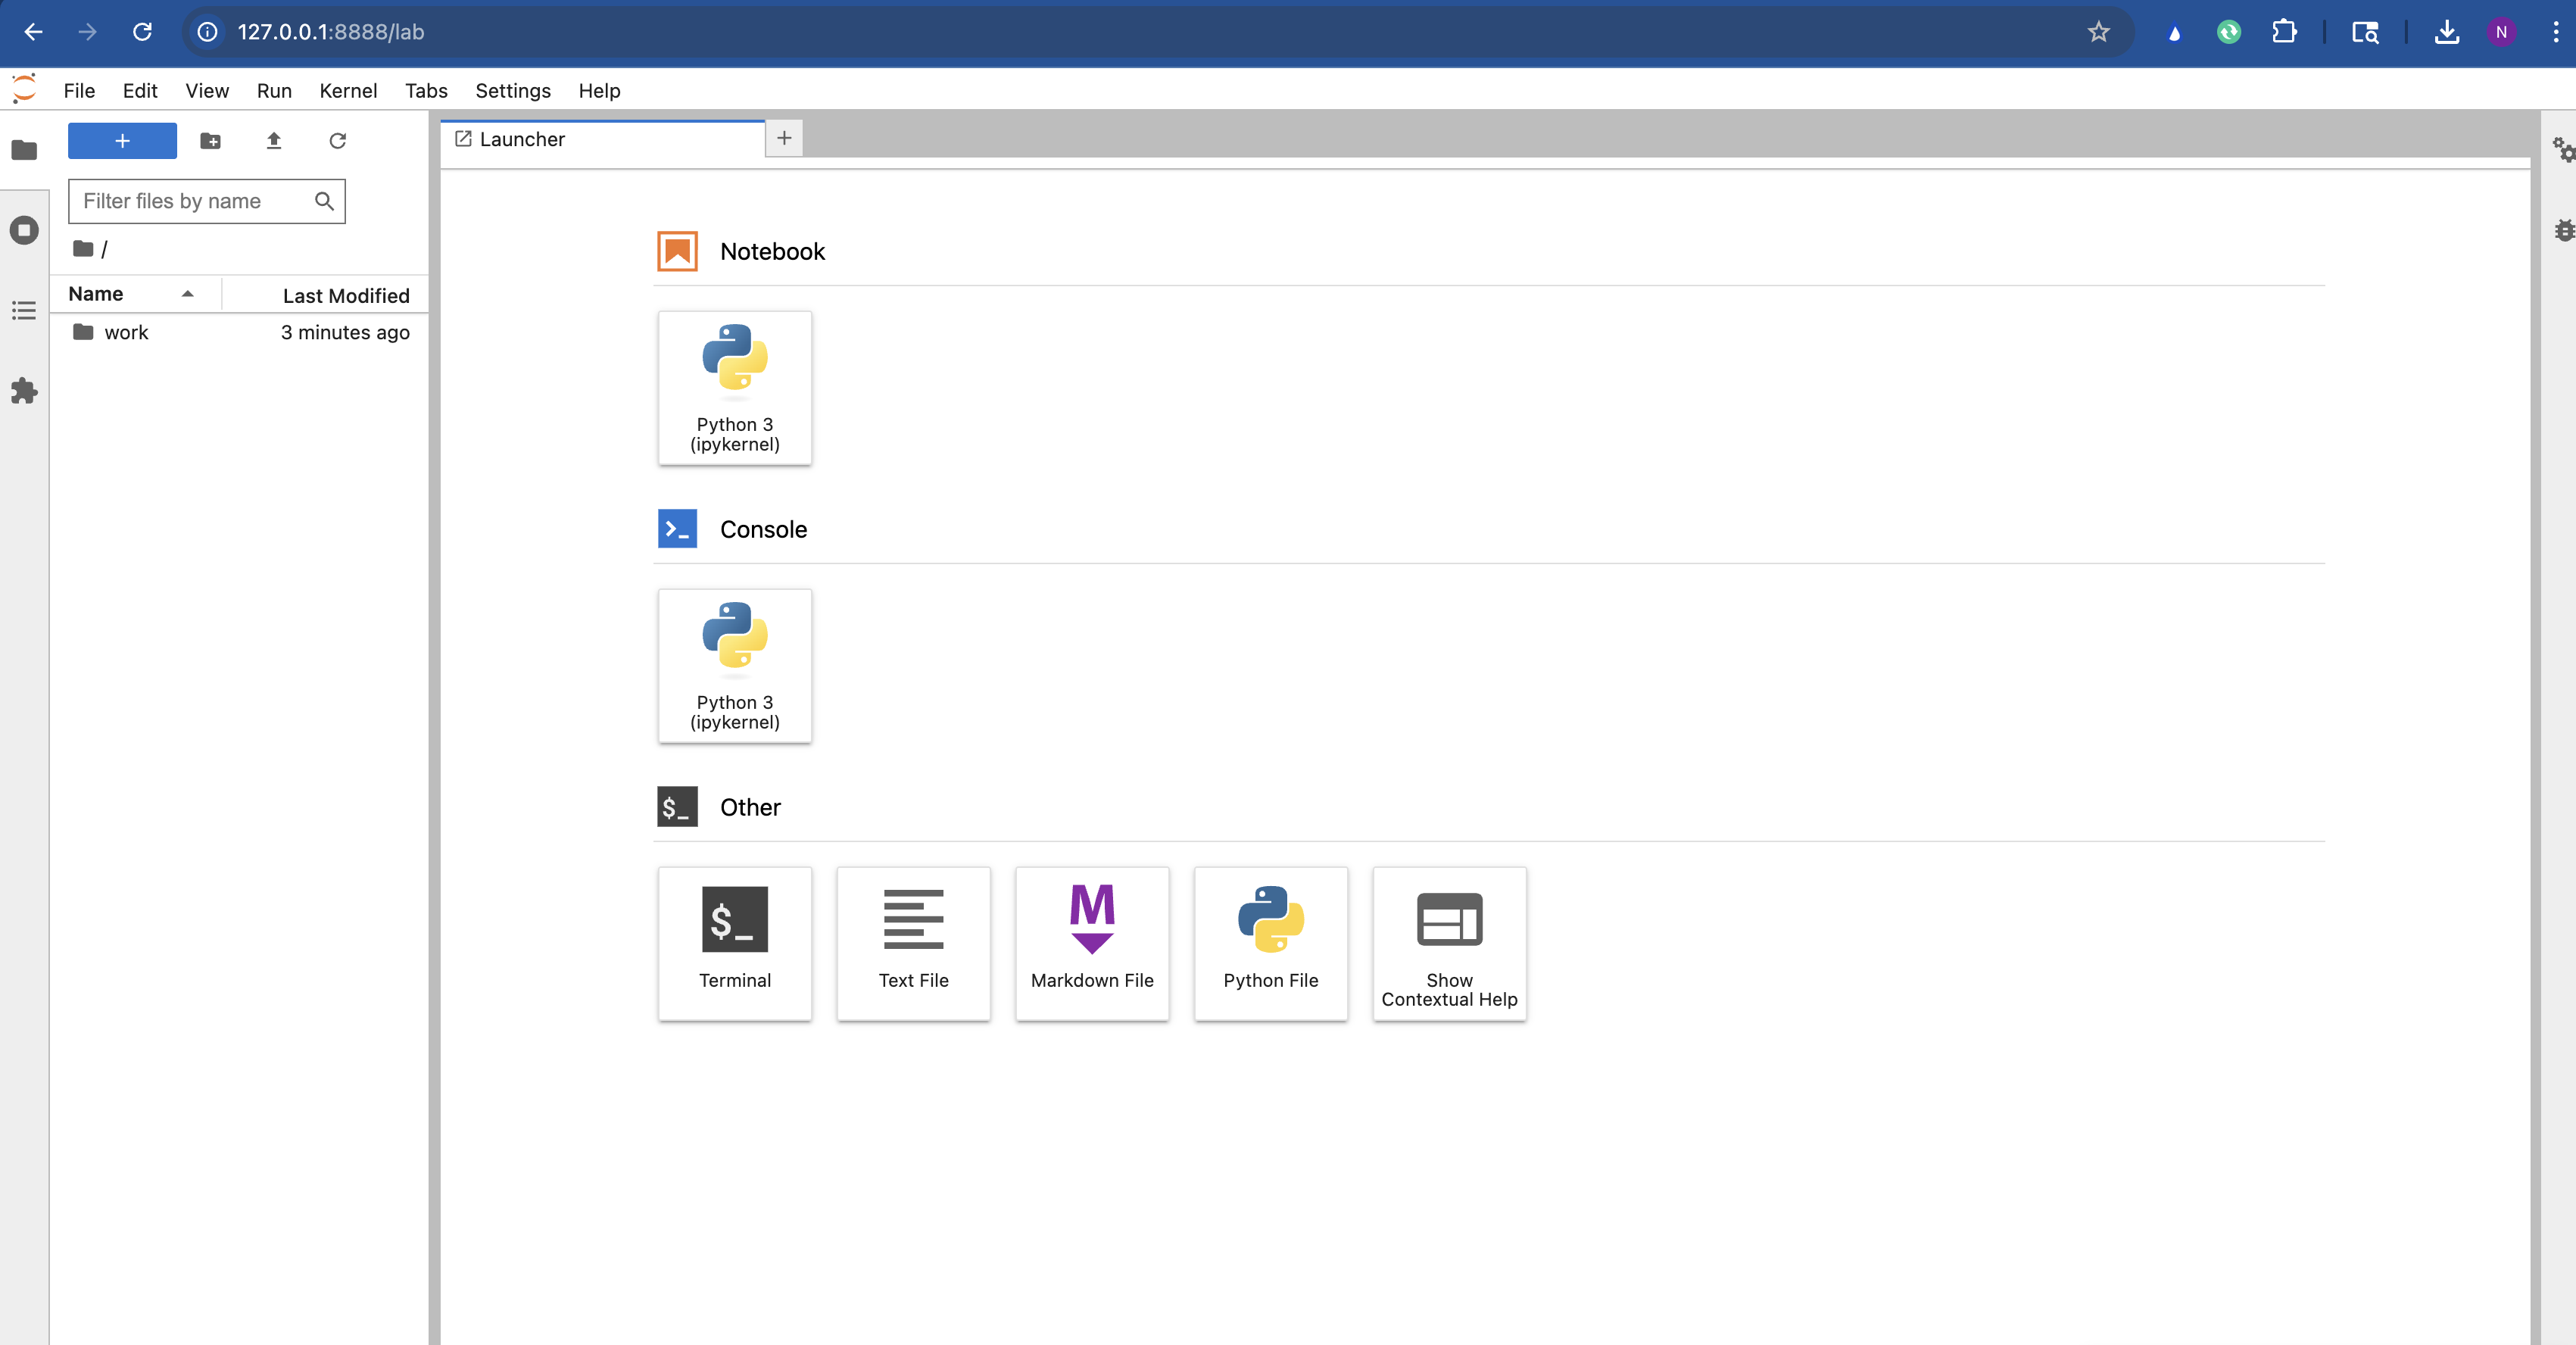
\includegraphics[width=0.95\textwidth]{images/step_7_2.png}
    \caption{Jupyter Lab interface running in browser at localhost:8888}
\end{figure}

\subsection{Explanation}
Successfully pulled the Jupyter Docker image (\texttt{jupyter/minimal-notebook:latest}) and started a Jupyter Lab server running in a Docker container. The container is running with port 8888 exposed and the umd\_classes directory mounted as a volume at \texttt{/home/jovyan/work} for easy access to course files. The Jupyter Lab interface is accessible at \texttt{http://127.0.0.1:8888} with the generated authentication token, demonstrating that Docker can successfully run complex applications with web interfaces and volume mounts.

\newpage

% Step 8
\section{Final Verification Commands}

\subsection{Objective}
Execute a series of verification commands to confirm all tools and configurations are working correctly.

\subsection{Commands Executed}
\begin{verbatim}
docker pull hello-world
docker --version
docker images
git pull
git status
git branch
python3 --version
\end{verbatim}

\subsection{Screenshot}
\begin{figure}[H]
    \centering
    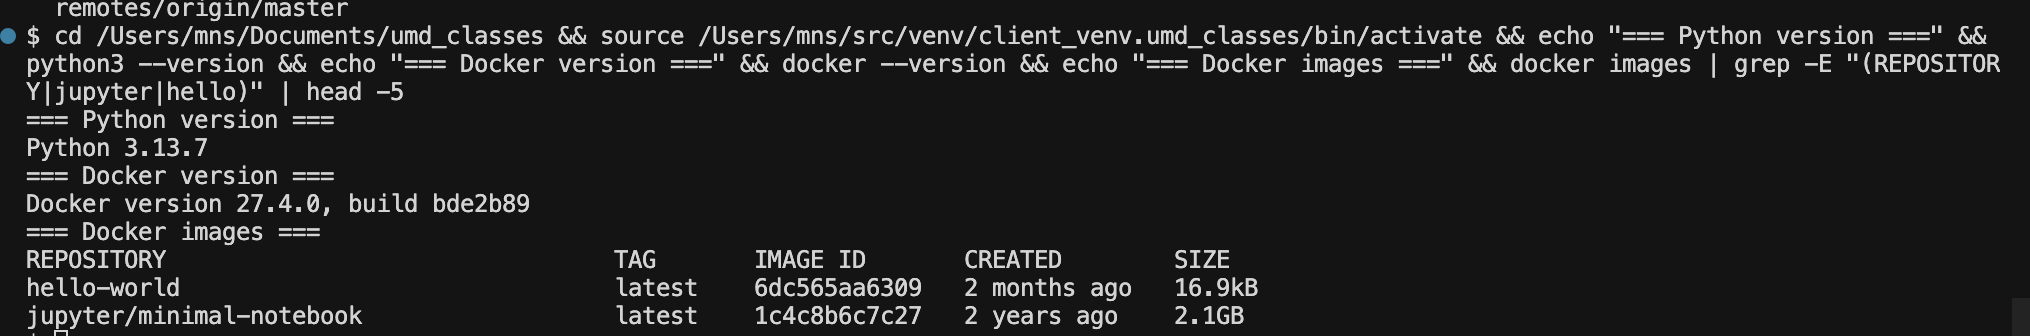
\includegraphics[width=0.95\textwidth]{images/step_8.png}
    \caption{Comprehensive verification of all development tools}
\end{figure}

\subsection{Explanation}
All verification commands executed successfully, confirming the complete development environment setup:

\begin{itemize}
    \item \textbf{Docker:} Successfully pulls images and manages containers (version 27.4.0)
    \item \textbf{Git:} Operations work correctly with repository up to date on master branch
    \item \textbf{Python:} Virtual environment active with Python 3.13.7
    \item \textbf{Images:} Both hello-world test image and jupyter/minimal-notebook available
\end{itemize}

This validates that all components of the development stack are properly configured and functional for course project work.

\newpage

% Conclusion
\section*{Conclusion}
\addcontentsline{toc}{section}{Conclusion}

This assignment successfully demonstrated the complete setup of a professional development environment for MSML610 coursework. All required components have been installed, configured, and verified:

\begin{enumerate}
    \item \textbf{GitHub Authentication:} SSH keys and Personal Access Tokens configured for secure repository access
    \item \textbf{Repository Management:} Course repository cloned with all submodules and helper libraries
    \item \textbf{Python Environment:} Isolated virtual environment with necessary dependencies
    \item \textbf{Docker Platform:} Containerization platform operational with ability to run complex applications
    \item \textbf{Jupyter Lab:} Interactive development environment running in containerized setup
\end{enumerate}

\vspace{0.5cm}
\noindent This environment is now ready for:
\begin{itemize}
    \item Running data analysis and machine learning workflows
    \item Developing and testing Python applications in isolated containers
    \item Collaborating on projects through version control
    \item Managing dependencies and ensuring reproducible results
\end{itemize}

\vspace{1cm}
\noindent\textbf{System Configuration Summary:}
\begin{table}[H]
\centering
\begin{tabular}{|l|l|}
\hline
\textbf{Component} & \textbf{Version/Details} \\
\hline
Operating System & macOS 24.6.0 (Darwin) \\
Docker & 27.4.0, build bde2b89 \\
Python & 3.13.7 \\
Git & Configured with SSH authentication \\
Virtual Environment & client\_venv.umd\_classes \\
Jupyter Lab & Running in Docker container \\
\hline
\end{tabular}
\end{table}

\end{document}

